\documentclass[../main]{subfiles}
% \ifSubfilesClassLoaded{
%     \dominitoc
%     %\externaldocument{../main.tex}   
% }{}

\begin{document}
\graphicspath{{./figures}}
\chapter{Architectures de cartes auto-organisatrices comme moyen de trouver de nouvelles formes d'apprentissage}
\minitoc
\section{Les cartes auto-organisatrices de Kohonen}\label{sec:som001}

Dans cette thèse, nous nous intéressons particulièrement aux \emph{cartes auto-organisatrices}, abrégées par SOM (Self-Organizing Maps). Le modèle de cartes auto-organisatrice a été initialement développé par Kohonen \cite{Kohonen1982}; le terme de cartes de Kohonen est ainsi utilisé pour désigner ce modèle initial. De nombreux modèles dérivés ont ensuite été développés à partir de ce modèle initial, sur diverses applications. On décompte par exemple plus de 11000 travaux utilisant les cartes de Kohonen dans la littérature en 2010(citer biblio).
Applications ?
Aspect topologique
Aspect local + variantes de SOM locales

\subsection{Carte de Kohonen classique}
Une carte de Kohonen est un algorithme de quantification vectorielle, cherchant à résumer un ensemble de données d'entrées issues d'un espace $\mathcal{D}$ en un nombre fini de vecteurs représentatifs, des prototypes.  Dans l'algorithme de Kohonen, ces prototypes sont disposés sur les noeuds d'un graphe, en général une grille en deux dimensions. Ce graphe est appelé carte de Kohonen. Les noeuds du graphe possèdent donc chacun un prototype et sont \emph{indexés}. Une distance entre noeuds est ainsi définie.
Au début de l'apprentissage, les prototypes ont une valeur aléatoires dans l'espace d'entrée. L'apprentissage est ensuite réalisé en trois étapes:
\begin{enumerate}
\item Une entrée $\inpx$ est présentée à la carte.
\item Le noeud ayant le prototype le plus proche de $\inpx$ selon une distance $d$, généralement la distance euclidienne, est choisie comme \emph{Best Matching Unit} (BMU) de la carte. Son index est notée $\bmu$.
\item Le prototype de la best matching unit est déplacé vers l'entrée $\inpx$, ainsi que les prototypes des noeuds voisins de $\bmu$ dans un rayon de voisinage défini à l'avance. On peut voir cette étape comme le déplacement d'une zone de la carte centrée en $\bmu$.
\end{enumerate}

L'algorithme de Kohonen repose donc sur à la fois un processus de compétition, avec la selection de la BMU de la carte, et un processus de coopération avec le déplacement des unités voisines de la Best Matching Unit et non seulement de cette dernière.
Toutes les données d'entrées sont tirées dans un même espace $\mathcal{D}$; par contre, la dimension de cet espace peut être quelconque.
L'apprentissage d'une carte de Kohonen se traduit par un rapprochement de tous les prototypes des données, de façon à ce que n'importe quel vecteur soit proche d'au moins un prototype. Visuellement, cela correspond à un dépliement de la carte dans l'espace d'entrée. On parlera donc de \emph{dépliement} d'une carte lorsque qu'on parle d'apprentissage. Ce dépliement est représenté en figures \ref{fig:som2d} et \ref{fig:som1d} pour des exemples de cartes en une et deux dimension, se dépliant sur des données en deux dimensions. 
A la fin de l'apprentissage, la carte conserve la structure topologique des données:
\begin{itemize}
\item Elle conserve les distances: deux prototypes ayant une distance proche dans la carte seront également proches selon la distance définie dans l'espace d'entrée. On observe donc une contiuité des valeurs des prototypes au sein de la carte
\item Elle conserve les densités. Une zone de $\mathcal{D}$ présentant plus de vecteurs aura plus d'unités la représentant dans la carte qu'une zone moins dense.
\end{itemize}
Par son aspect ordonné, une carte est une représentation en faible dimension d'un espace d'entrée de grande dimension. Les cartes de Kohonen sont ainsi utilisées dans de nombreuses applications, notamment pour visualiser des données de grande dimension et faire du regroupement de données (clustering). 

La carte de Kohonen est d'inspiration biologique. Le but premier de Kohonen était de développer un modèle informatique inspiré de l'organisation spatiale des neurones dans le cortex humain, dont un exemple est présenté en figure~\ref{fig:v1}. Il s'est notamment inspiré de l'organisation du cortex en colonnes corticales, ensemble de neurones réagissant à un même stimulus.

% \draft{
% (Kohonen book 1995)
% In an attempt to implement a learning principle that would
% work reliably in practice, effectively creating globally ordered maps of various
% sensory features onto a layered neural network, this author formalized the
% self-organizing process in 1981 and 1982 into an algorithmic form that is
% now being called the Self-Organizing (Feature) Map (SOM) [2.27 -29J. In the
% pure form, the SOM defines an "elastic net" of points (parameter, reference,
% or codebook vectors) that are fitted to the input signal space to approximate
% its density function in an ordered way. The main applications of the SOM
% are thus in the visualization of complex data in a two-dimensional display,
% and creation of abstractions like in many clustering techniques.

% Motivations de Kohonen: capacité des régions du cerveau à s'auto organiser. Note que certes il doit y avoir un prédetermination génétique, mais qu'on observe une réorganisation des mapping lors de déficiences par ex. 

% find abstract self-
% organizing processes in which maps resembling the brain maps are formed,
% whereas it is of less interest whether the maps are formed by evolution, post-
% natal growth, or learning.

% }

\begin{figure}
\centering
\includegraphics[width=0.5\textwidth]{digits.jpg}
\caption{Représentation de la base de données MNIST, images de chiffres écrits à main levées, par une SOM en deux dimension. Une continuité est observée dans la forme des images lorsqu'on se déplace dans la carte: le $0$ se transforme en $6$, etc.}
\label{fig:SOM}
\end{figure}



\subsection{Aspect topologique de la carte de Kohonen}

La carte de Kohonen se distingue d'autres algorithmes de quantification vectoriel par la topologie introduite par la carte dans l'ensemble des prototypes. Cette topologie dépend du voisinage utilisé par l'algorithme et de la dimension du support de la carte.
La plupart des algorithmes de SOM de la littérature utilisent comme support une grille en deux dimensions. L'indexation des noeuds est alors un ensemble de positions 2D.


En théorie, les cartes peuvent être une dimension (ligne), deux dimensions (grilles), ou de dimension plus grandes. Les cartes peuvent aussi être des graphes de forme plus variable. En pratique, les grilles deux dimension sont les plus couramment utilisées. Elles permettent d'effectuer une réduction de dimension, tout en étant facile à visualiser sur un écran. Les cartes de dimensions supérieures sont très rarement utilisées dans la littérature. Le cout de l'algorithme d'apprentissage dépend en effet du nombre de neurones, et celui-ci augmente exponentiellement lorsqu'on augmente la dimension d'une carte de Kohonen en plus de deux dimensions. Les calculs deviennent rapidement couteux, alors qu'un avantage de la carte de Kohonen est la simplicité et la rapidité de l'algorithme. Les cartes une dimension sont quant à elles limitées en terme de représentation des données, et sont donc rarement utilisées en pratique. Cependant, elles se prêtent bien à la représentation graphique. Nous utiliserons donc principalement des cartes en une dimension dans cette thèse.


De plus, les calculs et l'organisation générés par l'algorithme de Kohonen sont complexes déjà avec des cartes en une dimension. Leur description mathématique a été réalisée en \cite{cottrell_theoretical_2016,cottrell_theoretical_1998,fort_soms_2006}. La preuve de la convergence d'une carte a été réalisée seulement pour des cartes 1D et n'est pas généralisable directement au cas en deux dimensions. Les processus intervenant dans dans cartes 1D sont donc déjà mathématiquement difficiles à formaliser, difficulté qui augmente fortement avec les dimensions. Comme nous étudions dans cette thèse un nouveau modèle et cherchons à comprendre les mécanismes qui y interviennent, l'utilisation de cartes 1D réduit un peu la difficulté du problème. 
Les cartes de forme autre que 1D ou 2D sont moins couramment utilisées, mais peuvent avoir des avantages. On peut observer par exemple des cartes structurées en arbre \cite{koikkalainen_self-organizing_1990}, permettant une recherche de BMU structurée. Certains modèles construisent une carte de Kohonen noeud à noeud, donnant au final une carte de Kohonen sous forme d'un graphe construit par l'algorithme, telle que \cite{alahakoon_dynamic_2000}. 
\begin{figure}
\centering
\includegraphics[width=0.8\textwidth]{soms_topologies}
\caption{Exemples de connexions dans le graphe support d'une SOM. Deux noeuds sont connectés s'il sont à une distance de une unité. Les SOM en deux dimensions sont les plus communément utilisées dans la littérature, sous forme d'une grille ou d'une grille hexagonale. Les SOM une dimension sont également utilisées.}
\label{fig:topo}
\end{figure}

\begin{figure}
\centering
\includegraphics[width=0.7\textwidth]{som2d}
\caption{Dépliement d'une SOM 2D sur des données dans le plan $[0,1]^2$, \cite{Kohonen1995SelfOrganizingM} \label{fig:som2d}}

\end{figure}

\begin{figure}
\centering
\includegraphics[width=0.7\textwidth]{som1d}
\caption{Dépliement d'une SOM 1D sur des données dans un triangle 2D \cite{Kohonen1995SelfOrganizingM}\label{fig:som1d}}

\end{figure}

\subsection{Inspiration Biologique d'une carte de Kohonen}

Le développement des cartes par Kohonen est intiallement inspiré par les cartes topologiques observées dans le cerveau. En effet, si on cartographie la position des neurones par rapport aux stimuli auxquels ils répondent dans certaines zones sensorielles du cerveau, on observe une disposition ordonnée. Les neurones proches réagissent à des stimuli proches. Un exemple est ainsi celui du cortex visuel v1, représenté en figure~\ref{fig:v1}. L'aire associée à l'audition présente aussi une organisation topographique (tonotopic maps), ainsi que de nombreuses autres aires, sensorielles ou plus abstraites [ref kohonen book].

\begin{figure}
\centering
\includegraphics[width=0.6\textwidth]{v1.jpg}
\caption{Représentation des réponses du cortex visuel V1 à un stimulus visuel (batonnets d'orientation spatiale différentes). Les neurones répondant à une certaine orientation sont affichés de la même couleur. On observe une continuité entre les neurones proches dans le cortex et l'orientation à laquelle ils répondent. Cette propriété d'organisation est l'inspiration biologique des cartes de Kohonen. }
\label{fig:v1}
\end{figure}

\section{Les cartes de Kohonen comme modules d'une architecture d'apprentissage complexe ? }

Cette thèse se place dans une démarche de construire un modèle d'architecture permettant un calcul émergent, à partir de cartes auto-organisatrices.
Les cartes auto-organisatrices ont été largement étudiées depuis leur introduction en 1984. On dénombre de milliers de papiers en traitant, rien que sur la période 1984 - 2003 pour laquelle une bibliographie exhaustive par mot clés a été menée par Lampinen et Oja (ref). (De nombreux papiers ont été publiés depuis, 10000 selon une recherche par mot clés sur google scholar.)

La question d'architecture de cartes de Kohonen a été explorée. Associer les cartes en modèle hiérarchique faisait même partie des premiers travaux publiés autour des cartes de Kohonen.
L'association de quelques cartes de Kohonen dans des applications spécifiques est également assez répandue:
(citer association de cartes pour détection d'erreur, autres applis ?). Tous ces modèles sont des constructions adaptées pour résoudre un problème de machine learning spécifique.
Mais étonnament peu de travaux, par rapport à la littérature sur le sujet, se sont intéressés à l'association de cartes en tant que nouveau modèle à part entière.

Dans cette section, nous passons en revues les modèles existantes permettant, d'une façon ou d'une autre, de connecter des cartes entre elle. Nous étudierons d'un coté les modèles d'architectures de plusieurs cartes communiquant via des interfaces; nous étudierons également les modèles de cartes récurrentes. Les cartes récurrentes sont appliquées à des motifs temporels et ont la caractéristique d'utiliser des éléments de leur état passé pour calculer leur état à un instant donné. La notion de communication est ici encore présente et peut nous servir d'inspiration pour développer une architecture de cartes. Par ailleurs, nous avons mentionné que le traitement de données temporel doit pouvoir être intégrée dans une architecture de carte visant à être autonome. Il s'agit ici de trouver une méthode d'interface entre carte qui puisse à la fois connecter des cartes auto-organisatrices et introduire des connections récurrentes dans le temps. 

\subsection{Inspiration biologique}
Nous avons vu d'un coté que les cartes auto-organisatrices sont d'inspiration biologique; sans chercher à modéliser les neurones du cerveau, on tend vers des principes généraux rappelant ce qu'on peut observer dans le cerveau. De la même façon, on observe dans le cerveau de multiples aires communiquant entre elles. Cette communication est observée en biologie lorsque des neurones d'une aire cérébrales activent des neurones d'une autre aire cérébrale. 
Ces connexions à l'échelle des aires cérébrales peuvent être rétroactives, c'est à dire que l'activation entre deux zones se fait dans les deux sens. Par exemple, \cite{primate_cortex_91}: zones dans le cortex du primate. La plupart des connexions est établie dans les deux sens.

La notion d'aire cérébrale renvoie à un aspect modulaire du cerveau. Modules préexistants mais flexibles: ainsi certaines zones qui s'avèrent non utilisées, suite par exemple à la perte d'un sens, se voient réorganisées au profit d'autre zones. On peut donc relier le cerveau à un modèle modulaire, avec des modules apprenant et pouvant se réorganiser.

Ainsi, de la même façon que les cartes auto-organisatrices rappellent l'organisation du cerveau sans chercher à le modéliser, l'architecture biologique observé dans le cerveau justifie l'idée de créer des architectures modulaires de cartes auto-organisatrices. Quitte à imiter la biologie, autant le faire jusqu'au bout.

On peut explorer plus en détail la notion de modules dans le cerveau. Des zones sont directement liées à des entrées externes, des zones sensorielles, de bas niveau. Le cerveau présente ensuite  d'autres aires liées à ces zones sensorielles, qui apportent de plus en plus d'abstraction dans les représentations des sens. Des aires sont aussi dédiées à l'assocation de plusieurs aires. On parle alors d'architecture hiérarchique, en référence à cette structure de zones sensorielles vers zones abstraites. Cependant, des connexions entre aires peuvent exister dans les deux sens. 

\draft{Le modèle de ces connexions n'est pas établi, mais plusieurs hypothèses et modèles existent en neurosciences computationnelles pour chercher à comprendre ce phénomène. Les plus répandues sont la zone de convergence divergence et la réentrée. A mettre dans modèle computationnels}

\subsection{Systèmes autonomes de cartes auto-organisatrices}

Un des enjeux de l'intelligence artificielle est de construire des systèmes autonomes, en robotique par exemple. Les cartes auto-organisatrices ont déjà comme avantage d'être un modèle d'apprentissage non-supervisé: l'ensemble des neurones et des poids réagit aux données présentées pour en dégager des représentations, sans intervention ou retour extérieur. Ensuite s'arrête l'aspect autonome: l'utilisation des cartes pour des tâches applicative nécessite une intervention extérieure. Il faut par exemple étiquetter les poids pour pouvoir faire de la classification d'entrées. La reconstruction d'image utilise la carte comme donnée pour faire du post processing de reconstruction. Utilisée comme algorithme de machine learning, la carte n'est pas un système autonome. 

Kohonen écrivait ainsi dans son livre à propos des enjeux des cartes de Kohonen en 1995:


\begin{quote}Systems of SOMs. A far-reaching goal in self-organization is to create
autonomous systems, the parts of which control each other and learn from
each other. Such control structures may be implemented by special SOMs;
the main problem thereby is the interface, especially automatic scaling of
interconnecting signals between the modules, and picking up relevant signals
to interfaces between modules. We shall leave this idea for future research. \cite{Kohonen1995SelfOrganizingM}
\end{quote}
L'idée d'un système de SOMs s'inscrit dans une recherche de système autonome. En introduisant des connexions entre cartes, on autorise le système à s'auto-activer au lieu de simplement réagir à des entrées, ce qui est nécessaire pour créer un système dynamique. Nous chercherons donc à créer un système de SOMs qui réagit à des entrées, mais qui peut ensuite s'auto-activer.

\subsection{Notion de mémoires}

De la même manière que les aires du cerveau, on observe différent types de mémoires interagissant dans un cerveau: mémoire épisodique, mémoire à long terme. Le temps et la mémoire est en quelque sorte spacialisé grâce aux échelles et aux temps de connexions dans le cerveau. 
La notion de mémoire se rapporte finalement aux architectures et systèmes autonomes. Les mêmes éléments de cerveau sont utilisés dans des cadre sensoriels et de mémoire. 
Des systèmes autonomes doivent présenter une mémoire. 
La notion temporelle a donc tout intéret à être intégrée à une architecture de cartes auto-organisatrices dans le cadre de rechercher des systèmes plus autonomes.


\section{Architectures de cartes}

Quelques arhcitectures de cartes ont été développées dans la littérature depuis le développement des SOMs.  L'idée est de comparer les différents modèles afin d'avoir une vision générale des structures de SOMs existantes. Nous abordons ces modèles d'un point de vue structurel: comment s'effectue l'interface entre les cartes, et de quelle manière cet apprentissage est réalisé. 

\subsection{Architectures hiérarchiques de cartes}

Dès les début du développement des SOMs dans les années 90 par les travaux de Kohonen \cite{Kohonen1982,Kohonen1995SelfOrganizingM}, des travaux proposent des architectures à base de cartes auto-organisatrices \cite{LampinenClusteringPO,miikkulainen_script_1992,ritter_combining_1989}. L'enjeu d'associer des cartes auto-organisatrices est également une perspective envisagée par Kohonen dans ses travaux.
Ces architectures sont présentées comme des cartes auto-organisatrices \emph{hiérarchiques} par leurs auteurs. 
Cette hiérarchie désigne une architectures de “SOM de SOM”.
Ils visent à amélorier la capacité de classification et clustering d'une SOM classique, ce qui est montré dans leurs expériences.
En comparant ces deux travaux, on peut noter que l'architecture HSOM est plus générique que l'arhcitecture proposée en Mikkulaienn, qui est elle spécialement concue pour répondre à la reconnaissance du langage. Nous nous attarderons plus spécifiquement sur ces modèles génériques.

Parmi ces modèles d'architecture, nous pouvons identifier plusieurs mécanismes d'interface entre cartes.
Un grand nombre de travaux s'appuie sur une architecture qu'on peut qualifier de "selective", dont le principe général est illustrée en figure \ref{fig:hsom_selective}.
Dans une architecture hiérachiques, l'activation, le BMU d'une carte d'un niveau au sein de la hiérarchie permet de selectionner une carte d'un niveau suivant. Chacune des cartes du niveau suivant est alors entrainée sur un sous-ensemble des données d'entrées. Ce type d'apprentissage est réalisé niveau par niveau: les cartes d'un même niveau sont entièrement entraînées, puis les cartes du niveau suivant y sont ajoutées et entrainées à leur tour. On ne touche alos plus au premier niveau. 
Ce procédé est retrouvé dans \cite{barbalho_hierarchical_2001,suganthan_pattern_2001,miikkulainen_script_1992,dittenbach_growing_2000,ordonez_hierarchical_2010,zhao_stacked_2015}. L'application des modèles cités est différente, mais le procédé est similaire dans tous ces travaux.
La selection d'une carte pour le niveau suivant repose par exemple sur la position du BMU \cite{barbalho_hierarchical_2001}, une connexion neurone à neurone \cite{??}, ou encore un filtre appliqué sur l'entrée \cite{zhao_stacked_2015}.

\begin{figure}
    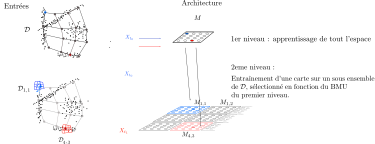
\includegraphics[width=\textwidth]{HSOM_selective.pdf}
    \caption{Exemple d'architecture hiérarchique sélective. La carte du premier niveau est entraînée sur tout l'espace d'entrée. Après apprentissage, la carte permet de filtrer les entrées pour les renvoyer vers une carte du niveau suivant. Dans cet exemple, la position du BMU de la carte du niveau 1 permet de sélectionner une carte du niveau 2, comme c'est le cas en \cite{barbalho_hierarchical_2001}. 
    L'entrée permet d'entraîner une carte du deuxième niveau. Chacune des cartes du niveau 2 apprend alors sur un sous-espace d'entrée.\label{fig:hsom_selective}}
\end{figure}

Travaux entre 2000 et 2010:
\cite{suganthan_pattern_2001,dittenbach_growing_2000,yamaguchi_adaptive_2010,ordonez_hierarchical_2010,barbalho_hierarchical_2001,gunes_kayacik_hierarchical_2007,wang_comparisonal_2007}


Enfin, on trouve un regain de publications sur les architectures de cartes auto-organisatrices sont publiés après 2015, cette fois sous la terminologie de “Deep SOM”. S'inspirant des réseaux de neurones profonds (deep learning), ayant connu un fort développement dans les années 2010 \cite{lecun_deep_2015}; ces travaux s'intéressent à l'apprentissgage d'image par des SOMs. 
\cite{Liu2015DeepSM,hankins_somnet_2018,wickramasinghe_deep_2019,aly_deep_2020,sakkari_convolutional_2020,dozono_convolutional_2016,nawaratne_hierarchical_2020,mici_self-organizing_2018}
L'arhcitecture Deep SOM est directement liée à HSOM: on prend les positions des BMUs pour apprendre le niveau suivant. Alors que HSOM proposaient une connexion d’une carte à une autre, DSOM prend un vecteur de positions de BMU en entrée, correspondant au BMU de chaque carte deu niveau inférieur.
On peut noter plusieurs travaux ayant implémenté et étendu DSOM sur diverses applications.
Remplacer cette section par : convsom vs selective som vs hsom

Enfin, un dernier type d'architecture hiérarchique de Soms se détache : les "Som convolutionnelles". Appliquée spécifiquement au traitement d'images, elles n'en sont pas moins des asssemblages de cartes. Dans ces archis \cite{Liu2015DeepSM,dozono_convolutional_2016}
On note que \cite{Liu2015DeepSM} utilise les positions des BMU comme entrée intermidaire d'une carte, alors que les autres utilisent l'entrée filtrée. Dans ce sens, L'architecture DSOM exploite vraiment l'aspect topologique d'une carte.

Dans tous ces cas, le but est que la couche finale du réseau possède de meilleurs perf en terme de classification que si on avait utilisé une SOM simple. Les cartes intermédiaires jouent le role de “routeurs” pour selectionner le BMU de la couche finale,  dont les paramètres sont mis à jour au cours de l'apprentissage.
Ces arhcitectures sont “feed forward”: DSOM, … , sont entrainées couches par couche, sans rétro action entre elles. 
Les expériences décrites dans cette biobliographie présentent les arhictetctures comme surpassant les capacité de classification d'une carte simple sur les jeux de données MNIST.
Aly ? evoque des perfs similaire à un réseau de deep learning supervisé
Note : pour une tache de classification, une carte peut eytre comparée à un algo supervisé: la phase de choix de la classe est gérée par un algorithme supervisé après entrainement de la carte.


Ces travaux montrent plusieurs choses:
Il existe différentes façon de transmettre des information entre couches. Les plus courantes sont la transmission de la position du BMU comme entrée pour la carte suivante, ou un caclul d'activation prenant en compte l'activitation de la couche précedente (connexion tous à tous).
La transmission de la position du BMU , notamment dans l'archi DSOM, montre que ce paradigme permet des bonne capacités de calcul + exploite l'aspect topologique des cartes.
- Ces arhcitectyures sont utilisées dans le meme cadre d'application que les SOMs classiques, pour notamment de la classification; les perf surpassent alors l'algo simple. Les travaux HSOM, DSOM notent ainsi une meilleure (plus fine ? ) séparation des classes. La présence de couche multiple a bien généré de nouveaux espaces de calcul et un Meilleur niveau d'abstraction. Ce niveau d'abstraction est pariculirètement utile dans le cadre de la reconnaissance d'images.

Comparaison des algos avec les SOMs et d'autres méthodes de classif (EM …) ???

C'est l'avenement du deep learning qui a poussé à créer des archi de SOMs. De la meme facon que les réseaux profonds ont étendu les capacités d'apprentissage du perceptron, les couhes de SOM montrent la meme ppté.
 Est-ce que la recherche actuelle sur l'apprentissage non supervisé poussera à remettre les SOM au gout du jour ? Est-ce qu'on ne fait pas de deep som, simplement parce que les outils n'ont pas été développés comme ceux du deep learning ? L'aspect non linéaire d'une SOM peut pourtant etre prometteuse dans ce cadre d'applis.

Il s'agit par contre d'archiectures completement feed forward: on ne peut pas vraiment parler d'archi modulaires.
On fera référence à ce type d'archis comme des archis hiérarchiques.

On peut mentionner le papier avec des cartes qui font un genre de backprop.


\begin{itemize}
    \item Historique de l'assemblage des SOMs en architectures feedforward ? 
    \item Quels sont les avantages apportés par les deep SOMs par rapport à des Soms classiques
    \item Quels sont les avantages des deep SOM par rapport aux réseaux de deep Learning 
    \item Pourquoi ne sont elles pas plus utilisées maintenant ?
\end{itemize}

\subsection{Strutures de cartes auto-organisatrices non-hiérarchiques}

De nombreux travaux de biologie observent des co-activations entre les zones du cerveaux. Le cortex cérébral est ainsi être considéré comme un reseaux de neurone modulaires, avec des régions s'activant entre elles. \cite{primate_cortex_91,mountcastle_columnar_1997,Harriger2012RichCO}

Ces coactivations aient été observées expérimentalement. Plusieurs modèles en neurosciences computationnelles ont été proposés pour expliquer ce phénomènes. Les modèles les plus communs sont la zone de convergence-divergence de Damasio (CDZ) \cite{damasio_time-locked_1989}, et le modèle de boucles de réentrées de Edelmann \cite{Edelman1982GroupSA}.

La zone de convergence divergence propose que certains réseaux de neurones dans le cerveau servent de connexions pour associer d'autres zones corticales. Lorsque cette zone est excitée par des signaux en provenance d'une zone corticale, elle propage cette excitation vers les autres zones.
La théorie de la ré-entrée postule quant à elle des connexions directes et réciproques entre  les neurones de différentes cartes cérébrales. Ces connexions permettent la coactivation de neurones dans différentes cartes. 

Par leur proximité avec la biologie, les travaux sur les réseaux de neurones impulsionnels ont été plus encleins à développer des modèles de cartes connectées, s'inspirant notamment des deux théories de convergence-divergence et de réentrée. Le fait que ces réseaux reposent déjà sur des calculs locaux les rendent de bons candidats pour créer des réseaux modulaires. En \cite{electronics9101605}, les auteurs passent en revue différents modèles implémentant de telles architectures au vu de leur plausibilité biologique, et proposent également une architecture de deux cartes auto-organisatrices impulsionnelles pour faire de la fusion de données.


Dans \cite{dominey13}, les auteurs construisent des architectures hiérarchiques en transmettant les positions des BMU entre les cartes multimodales. L'inspiration est tirée du cadre CDZ.
Chacune des cartes possède plusieurs couches, chacune prenant une modalité en entrée. Une activité est calculée sur ces modalités en une activité commune. La position du BMU, en l'occurence un vecteur 3D, sera utilisée comme modalité hiérachique pour connecter des cartes entre elle. Dans ces travaux, les auteurs présentent une architecture hiérarchique, en s'appuyant sur le modèle CDZ. Une carte amodale sert alors à connecter des cartes modales.
Dans le cas d'une hiérarchie de cartes, les auteurs entrainent les couches de l'architecture séparément: les cartes modales du premier niveau sont apprises, puis la carte amodale les connectant est apprise dans un second temps. 
Une fois toute les cartes apprises, la structure est utilisée pour activer une ou des modalités en activant la carte amodale. Cette carte représente la zone de convergence divergence des modèles cérébraux. 

\begin{figure}
    \centering
    \includegraphics[width=0.3\textwidth]{MMCM_schema.pdf}
    \caption{Architecture MMCM. Les cartes du premier niveau recoivent l'une les mouvements de tête d'un robot, l'autre les mouvements de main. Les cartes convergent en une carte amodale (MMCM). L'activation de cette carte produit des mouvements coordonées tête/mains~\cite{dominey13}\label{fig:mmcm}}
\end{figure}

ASOM
\cite{johnsson_associating_2008}


\subsection{Cartes auto-organisatrices récurrentes}

On appelle réseaux récurrents des réseaux de neurones qui prennent en compte leur état précédent pour calculer leur état actuel. Ces réseaux sont utilisés pour le traitement et l'apprentissage de signaux temporels. Citons par exemple, en deep learning, les RNN (recurrent neural networks), dont les neurones recoivent leur état précédent en entrée. Les réseaux récurrents les plus utilisés actuellement sont les LSTM, dans lesquel un système de portes perment d'activer ou non des neurones en fonction des états précédents du réseau. Les cartes de Kohonen ont elles aussi des version récurrentes que nous allons présenter dans cette partie.

Nous nous intéressons aux architectures multi-cartes, mais les cartes récurrentes répondent à des problèmes très similaire à ceux rencontrés dans la conception d'architectures de cartes pour faire de la mémoire associative. Dans une carte récurrente, le problème principal est de trouver comment communiquer à la carte de l'information sur son état précédent et comment utiliser cette information dans l'apprentissage de l'état courant. Cela rejoint la problématique posée dans les architectures de cartes de Kohonen, qui est de comment communiquer à une autre carte son état, afin de l'utiliser dans l'apprentissage de l'état courant. Nous avons vu précedemment qu'il existe assez peu de modèles d'architectures de cartes. Il existe plusieurs modèles de carte récurrentes qui nous permettrons de compléter cette étude. 

Notre volonté de créer un modèle général d'architecture de cartes auto-organisatrice motive également le fait de s'intéresser aux cartes récurrentes. On souhaite en effet créer un modèle qui puisse unir cartes récurrentes et cartes normales au sein d'une même architecture. L'aspect bio-inspiré du modèle et son aspect multimodal ciblent plutot des applications d'un tel réseau en robotique. Or, la plupart des données traitées par des réseaux de neurones, en particulier dans les applications robotiques, sont temporelles : vidéos, signaux sonores, capteurs de position. Il est donc important de s'appuyer autant sur les modèles de cartes récurrentes existantes que sur les architectures afin de créer un modèle général. 

%Enfin, les cartes de Kohonen ne se prêtent pas à un apprentissage en ligne de données en temps réel. En effet, il est nécessaires que les données d'entrées soient tirées aléatoirement dans l'espace à apprendre et ne suivent pas une trajectoire. Par exemple, si on veut apprendre des images, mais que les entrées sont données à la carte sous la forme d'une vidéo, les frames de la vidéo sont proches les unes des autres et forment donc une continuité dans l'espace d'entrée des images à apprendre. La carte va alors apprendre le sous ensemble de l'espace sur lequel se trouvent les premières frames, puis les oublier au fur et à mesure de l'apprentissage et les remplacer par les images qui suivent. Avec une architecture multi cartes qui prendrait en compte un aspect temporel, on pourrait imaginer la construction d'une architecture plus robuste.

Nous avons classé les modèles de cartes récurrentes existants en différentes catégories. D'une part, certains modèles de cartes utilisent l'état précédent de la carte lors du calcul de l'activité de l'état courant. De l'autre, des modèles réutilisent plutot des élement de la carte précedente en tant qu'entrée de l'état courant.



\subsubsection{The Hypermap architecture, TKM, RSOM}
Parmi les premiers travaux autour des cartes auto-organisatrices, Kohonen propose l'"Hypermap" \cite{Kohonen1991THEHA} L'idée de cette méthode est, pour une carte apprenant sur une séquence d'entrée, de présenter la carte une entrée et un contexte dépendant de l'état précédent. Ce contexte défnit une zone de la carte dans laquelle faire le matching.


\section{Axe de recherche choisi}

Nous avons détaillé la littérature existante en terme d'architecture de SOMs et plus généralement de réseaux de neurones auto-organisés. Nous avons divisé ces architectures en deux grandes catégories: un format hiérarchique et \emph{feedforward}, et un format non-hiéarchique incluant des rétroactions.
Le format feedforward implique généralement un apprentissage couche par couche. Ce format est très appliqué et permet d'amélorier les capacités de clustering d'une SOM classique, principalement dans le cas ou les données traitées présentent elles-mêmes une structure hiérarchique, telles que des images ou des phrases.
Nous cherchons à développer une architecture plus générale de cartes auto-organisatrices et ne nous placons ainsi pas dans le contexte des deep SOM mentionné ci-dessus. 
Cependant, nous notons que la position du BMU comme interface entre couche de cartes permet des capacités de calcul.
Nombre de ces architectures sont développées directement dans un but applicatif. On peut ainsi faire la distinction entre un modèle d'architecture, tel que HSOM, qui est générique et applicable à tout type de données, et une structure appliquée, développées spécifiquement pour un type de données.

Opposées à ces arhcitectures hiérarchiques, des architectures reposent sur de l'interaction entre cartes, avec des boucles de rétroaction.
Ces architectures sont moins présentes dans la littérature que les deep SOM, et cherchent en général à se rapprocher d'un contexte biologique, telle que CDZ dominey.
Nous nous placons plutot dans la lignées des cartes non-hiérarchiques, sans vouloir cependant copier un aspect biologique.
De façon intéressante, nous remarquons que plusieurs structures non hiérarchiques sont associées à l'apprentissage de données temporelles. Ces architectures se rapprochent des modèles appélés cartes auto-organisatrices récurrentes, dans lesquels des éléments de calcul d'une carte à une itération données sont réutilisés pour le calcul des itérations suivantes. Ces modèles permettent à une 


Dans cette thèse, nous cherchons à développer un modèle d'architecture non-hiérarchique de SOM. En effet, il semble que peu de travaux aient exploré l'idée d'associer des SOMs en architectures comportant des rétroactions, et non seulement en architecture hiérachiques. 
Une telle archi peut etre alors vue comme un système complexe dans lequel nous pouvons nous attendre à l'émergence possible de calcul par l'ensemble des cartes.
Les choix pour la construction d'une telle architecture se situent au niveau de l'interface entre cartes. De nombreux travaux autour des cartes de Kohonen utilisent la position du BMU comme vecteur de l'information transmise entre plusieurs cartes. 
Nous faisons ce choix également et nous utiliserons un

\ifSubfilesClassLoaded{
    \bib
    %\externaldocument{../main.tex}   
}{}
\end{document}